\chapter{Data Mining}\label{chap:data-mining}

\section{Things Useful to Know}\label{sec:things-useful-to-know}

\begin{enumerate}
    \item The \textbf{TF.IDF} (\textit{Term Frequency times Inverse Document Frequency}) measure of word importance.
    \item Hash functions and their use.
    \item Secondary storage (disk) its effect on running time of algorithms.
    \item The base $e$ of natural logarithm and identities involving that constant.
    \item Power laws.
\end{enumerate}

\subsection{Importance of Words in Documents}\label{subsec:importance-of-words-in-documents}

Classification often starts by looking at documents, and finding the significant words in those documents. Our first guess might be that the words appearing most frequently in a document are the most significant. However, that intuition is exactly opposite of the truth. The formal measure of how concentrated into relatively few documents are the occurrences of a given word is called \textbf{TF.IDF}. It is normally computed as follows. Suppose we have a collection of $N$ documents. Define $f_{ij}$ to be the \textit{frequency} of term (word) $i$ in document $j$. Then, define the \textit{term frequency} $\bm{TF}_{ij}$ to be:
\begin{equation*}\label{eq:tf}
    \bm{TF}_{ij} = \frac{f_{ij}}{\max_{k} f_{kj}}
\end{equation*}
That is, the term frequency of term $i$ in document $j$ is $f_{ij}$ normalized by dividing it the maximum number of occurrences of any term (perhaps excluding stop words) in the same document. 

The IDF for a term is defined as follows. Suppose term $i$ appears in $n_i$ of the $N$ documents in the collection. Then $\bm{IDF}_i = \log_2(N/n_i)$. The \textbf{TF.IDF} score for term $i$ in document $j$ is then $\bm{TF}_{ij} \times \bm{IDF}_i$.

\subsection{Hash Functions}\label{subsec:hash-functions}

A hash function $h$ takes a \textit{hash-key} value as an argument and produces a \textit{bucket number} as a result. The bucket number is an integer, normally in the range $0$ to $B - 1$, where $B$ is the number of buckets. Hash-keys can be of any type. There is an intuitive property of hash functions that they ``randomize'' hash-keys.

\subsection{Indexes}\label{subsec:indexes}

An \textit{index} is a data structure that makes it efficient to retrieve objects given the value of one or more elements of those objects. The most common situation is one where the objects are records, and the index is on one of the fields of that record. Given a value $v$ for that field, the index lets us retrieve all the records with value $v$ in that field.

\subsection{Secondary Storage}\label{subsec:secondary-storage}

Disks are organized into \textit{blocks}, which are the minimum units that the operating system uses to move data between main memory and disk. It takes approximately ten milliseconds to \textit{access} and read a disk block. That delay is at least five orders of magnitude (a factor of $10^5$) slower than the time taken to read a word from main memory. You can assume that a disk cannot transfer data to main memory at more than a hundred million bytes per second (100MB), no matter how that data is organized. That is not a problem when your dataset is a megabyte. But a dataset of a hundred gigabytes or a terabyte presents problems just accessing it, let alone doing anything useful with it.

\subsection{The Base of Natural Logarithms}\label{subsec:the-base-of-natural-logarithms}

The constant $e = 2.7182818...$ has a number of useful special properties. In particular:
\begin{equation*}
    \lim_{n \to \infty} \left(1 + \frac{1}{n}\right)^n = e
\end{equation*}

Some algebra lets us obtain approximations to many complex expression. Condiser $(1 + \alpha)^\beta$, where $\alpha$ a small. We can rewirte the expression as $(1 + \alpha)^{(1/\alpha)(\alpha\beta)}$. Then subsitute $\alpha = 1/n$ and $1/\alpha = n$, so we have that $(1+\frac{1}{n})^{n(\alpha\beta)}$, which is
\begin{equation*}
    \Bigg(\left(1 + \frac{1}{n}\right)^n\Bigg)^{\alpha\beta}
\end{equation*}
Since $\alpha$ is assumed small, $n$ is large, so the subexpression $\left(1 + \frac{1}{n}\right)^n$ will be cose to the limiting value of $e$. 

Some other usefull approximations follow from the Taylor expansion of $e^x$. That is,
\begin{equation*}
    \begin{split}
    e^x & = \sum_{i=0}^{\infty} \frac{x^i}{i!} \\
        & = 1 + x + \frac{x^2}{2!} + \frac{x^3}{3!} + \cdots
    \end{split}
\end{equation*}

When $x$ is large, the above series converges slowly, although it does converge because $n!$ grows faster than $x^n$ for any constant $x$.

\subsection{Power Laws}\label{subsec:power-laws}

There are many phenomena that relate two variables by a \textit{power law}, that is, a linear relationship between the logarithms of the variables. Figure~\ref{fig:power-law} suggest such a relationship that is: $\log_{10} y = 6 - 2\log_{10}x$

\begin{figure}[H]
\centering
\scalebox{0.8}{
\begin{tikzpicture}
    % Axes
    \draw[->] (0,0) -- (6,0) node[right] {$x$};
    \draw[->] (0,0) -- (0,8) node[above] {$y$};
    
    % Ticks and labels on x-axis
    \foreach \x/\label in {1/1, 2/10, 3/100, 4/1000, 5/10.000}
        \draw (\x,0.1) -- (\x,-0.1) node[below] {\label};
    
    % Ticks and labels on y-axis
    \foreach \y/\label in {1/1, 2/10, 3/100, 4/1000, 5/10.000, 6/100.000, 7/1.000.000}
        \draw (0.1,\y) -- (-0.1,\y) node[left] {\label};
    
    % Dotted line
    \draw[dotted] (0,7) -- (4,0);
\end{tikzpicture}
}
\caption{A power law with a slope of $-2$}
\label{fig:power-law}
\end{figure}

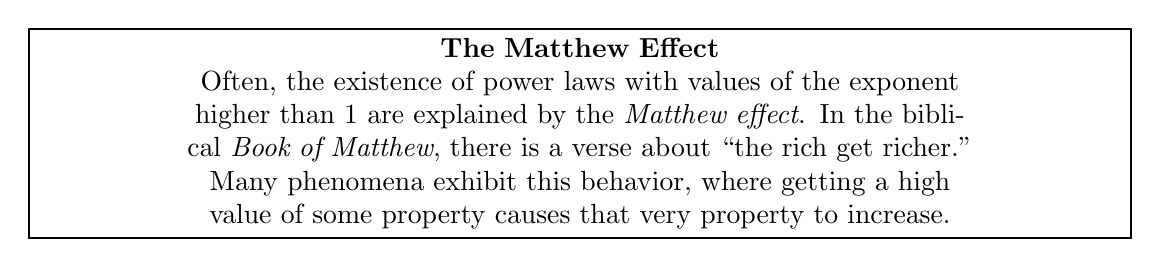
\begin{tikzpicture}
    \node [draw=black, thick, rectangle, minimum width=14cm, minimum height=2cm, align=center, text width=12cm] (box) {
        \textbf{The Matthew Effect} \\
        Often, the existence of power laws with values of the exponent higher than 1 are explained by the \textit{Matthew effect}. In the biblical \textit{Book of Matthew}, there is a verse about ``the rich get richer.'' Many phenomena exhibit this behavior, where getting a high value of some property causes that very property to increase.
    };
\end{tikzpicture}

